\documentclass{article}

%\usepackage[landscape, centering, showcrop=true]{geometry} %
\usepackage[
%layoutheight=297mm,layoutwidth=450mm,  %420+thickness--here 30mm; estimate n*0.1/2 with 80g papers
%layoutvoffset=25mm,layouthoffset=30mm,
%paperheight=347mm,paperwidth=510mm,
paperheight=320mm,paperwidth=450mm,
margin=30mm,showcrop=false]{geometry}
%\usepackage[pdflatex,cam,center,a3,height=35cm,width=47cm]{crop} %

\usepackage[utf8]{inputenc}
%\usepackage[T1]{fontenc}

%%% FONT PACKAGES
%\usepackage[scaled=0.85]{beramono} % inconsolata or beramono ???
%\usepackage{fouriernc} % serif: new century schoolbook
\usepackage{avant}     % sans serif: Avant Garde
\usepackage{microtype} % Slightly tweak font spacing for aesthetics
%\usepackage{changepage}   % for the adjustwidth environment to make narrow paragraphs

\usepackage{sectsty} %change font on headings
\allsectionsfont{\sffamily}


\usepackage{tikz}
\usetikzlibrary{calc}

\definecolor{Background}{HTML}{A10618}%{A10618}%
% lila90% {HTML}{411934} orange E95420 lila 2C001E D-rosa: F280A1
% red: {rgb}{0.7,0.07,0.12} vivid red: {HTML}{C90018}
\definecolor{Foreground}{HTML}{FFFFFF} % 000000 FFFFFF

\newcommand{\LibVersion}{0.1.0} % latest version of introlib at https://github.com/lunduniversity/introprog-scalalib
\newcommand{\LibJar}{\texttt{introprog-\LibVersion.jar}}
\newcommand{\JDKApiUrl}{\url{https://docs.oracle.com/javase/8/docs/api/}}


\begin{document}


\pagecolor{Background}
\color{Foreground}


\newcommand{\LeftMarginBack}{1.0}
\newcommand{\RightMarginFront}{1.0}
\newcommand{\YPosFront}{-1.5}
\newcommand{\YPosBack}{0}

\thispagestyle{empty}
\renewcommand{\familydefault}{\sfdefault}
\renewcommand{\arraystretch}{1.5}
%\newgeometry{a3paper,landscape, centering}
%\makeatletter\CROP@center\makeatother

\begin{tikzpicture}[overlay,remember picture]%[overlay,remember picture]
    %\fill[Pink,fill opacity=1.0] (current page.south west) rectangle (current page.north east);
    \node[text width=250mm, align=right] (intro) at ($(current page.north east)+(-14.5,-6.8)-(\RightMarginFront,\YPosFront)$) {
       \fontsize{28}{46}\sffamily\selectfont{Introduktion~~till}
       };

    \node[text width=250mm, align=right] (prog) at ($(current page.north east)+(-14.5,-8.5)-(\RightMarginFront,\YPosFront)$) {
       \fontsize{52}{46}\sffamily\selectfont\textbf{programmering}
       };

       \node[text width=250mm, align=right] (intro) at ($(current page.north east)+(-14.5,-10.0)-(\RightMarginFront,\YPosFront)$) {
          \fontsize{28}{46}\sffamily\selectfont{med~~Scala}
          };


    \node[text width=250mm, align=right] (prog) at ($(current page.north east)+(-14.5,-28.8)-(\RightMarginFront,\YPosFront)$) {
       \fontsize{28}{46}\sffamily\selectfont{DEL 1
       }
       };

    \node[text width=250mm, align=right] (prog) at ($(current page.north east)+(-14.5,-30.0)-(\RightMarginFront,\YPosFront)$) {
       \fontsize{18}{46}\sffamily\selectfont\texttt{http://cs.lth.se/pgk}
       };

    %\node[text width=250mm, align=right] (prog) at ($(current page.north east)+(-14.5,-28.2)$) {
    %   \fontsize{18}{46}\sffamily\selectfont  2016
    %   };


    %\node[above right] (picture) at ($(current page.north east)+(-16,-27.5)-(\RightMarginFront,\YPosFront)$)
     %{
\includegraphics[width=140mm]{gurka.jpg}};
    %\node[above right] (picture) at ($(current page.north east)+(-15,-25.5)-(\RightMarginFront,\YPosFront)$){
\includegraphics[width=120mm]{../../img/scala-logo}};
    \node[above right] (picture) at ($(current page.north east)+(-15,-25.5)-(\RightMarginFront,\YPosFront)$){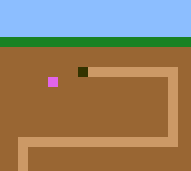
\includegraphics[width=120mm]{../../img/blockworm}};


\node[above right] (logo) at ($(current page.west)+(19.0,-21.8)+(2.5,0.5)$) {
\includegraphics[scale=0.54]{../../img/logoLUeng}};



\node[anchor=north,rotate=-90, align=left] (back) at ($(current page.north)+(0.0,-11.8)+(0,+2.0)$) {
\fontsize{18}{20}\sffamily\selectfont\textbf{Introduktion till programmering med Scala%
 %och Java
 }%\hspace{2.0cm}\texttt{http://cs.lth.se/pgk}
 };

\node[anchor=north] (back) at ($(current page.north)+(-0.4,-15.0)+(0,-6.3)$) {
\fontsize{16}{20}\sffamily\selectfont {\CurrentYear}};

\node[anchor=north] (back) at ($(current page.north)+(-0.4,-15.0)+(0,-7.3)$) {
\fontsize{16}{20}\sffamily\selectfont {DEL 1}};


\node[above right, scale=1.3] (modulplan) at ($(current page.west)+(\LeftMarginBack,-11.5)+(1.0,\YPosBack)$) {
\sffamily%!TEX encoding = UTF-8 Unicode
\begin{tabular}{l|l|l|l}
\textit{W} & \textit{Modul} & \textit{Övn} & \textit{Lab} \\ \hline \hline
W01 & Introduktion            & expressions & kojo            \\
W02 & Kodstrukturer           & programs    & --              \\
W03 & Funktioner, Objekt      & functions   & bugs            \\
W04 & Datastrukturer          & data        & pirates         \\
W05 & Sekvensalgoritmer       & sequences   & cards           \\
W06 & Klasser, Likhet         & classes     & turtlegraphics  \\
W07 & Arv, Gränssnitt         & traits      & turtlerace-team \\
KS  & KONTROLLSKRIVN.         & --          & --              \\
W08 & Mönster, Undantag       & matching    & chords-team     \\
W09 & Matriser, Typparametrar & matrices    & maze            \\
W10 & Sökning, Sortering      & sorting     & surveydata-team \\
W11 & Scala och Java          & scalajava   & lthopoly-team   \\
W12 & Trådar                  & threads     & life            \\
W13 & Design                  & Uppsamling  & Projekt         \\
W14 & Tentaträning            & Extenta     & --              \\
T   & TENTAMEN                & --          & --              \\
\end{tabular}

};

\node[above right, text width=15cm,align=left] (collection-traits) at ($(current page.west)+(\LeftMarginBack,3.8)+(1.0,\YPosBack)$) {
\begin{minipage}{1.0\textwidth}\sffamily\large
Detta kompendium är kurslitteratur i grundkursen i programmering på Datateknikprogrammet vid Lunds tekniska högskola.

\vspace{1em}
I kursen används det moderna och kraftfulla programmeringsspråket Scala för att illustrera grunderna i imperativ och objektorienterad programmering, samt elementär funktions-programmering.

\vspace{1em}
En viktig framgångsfaktor vid studier i programmering är din egen upptäckarglädje och experimentlusta. Du lär dig bäst genom att skapa dina egna program. Varje bugg du fixar i din egen kod fördjupar dina insikter.

\vspace{1em}
Läromaterialet fokuserar därför på lärande genom praktiskt programmeringsarbete och innehåller övningar och laborationer som är organiserade i moduler enligt en noga uttänkt progression, där dina kunskaper utvecklas steg för steg. Varje modul har ett tema enligt tabellen nedan.



\vspace{1em}
Välkommen till datavetenskapens fascinerande värld!
\end{minipage}
};

\node[above right, scale=1.3] (modulplan) at ($(current page.west)+(\LeftMarginBack,-13.5)+(1.0,\YPosBack)$) {
\begin{minipage}{0.33\textwidth}
\sffamily Datavetenskap, LTH, Lunds universitet. Licens: CC-BY-SA. Upplaga \CurrentYear. \\ \texttt{http://cs.lth.se/pgk}
\end{minipage}
};


%\node[above right] (collection-traits) at ($(current page.west)+(4.0,-9.5)$) {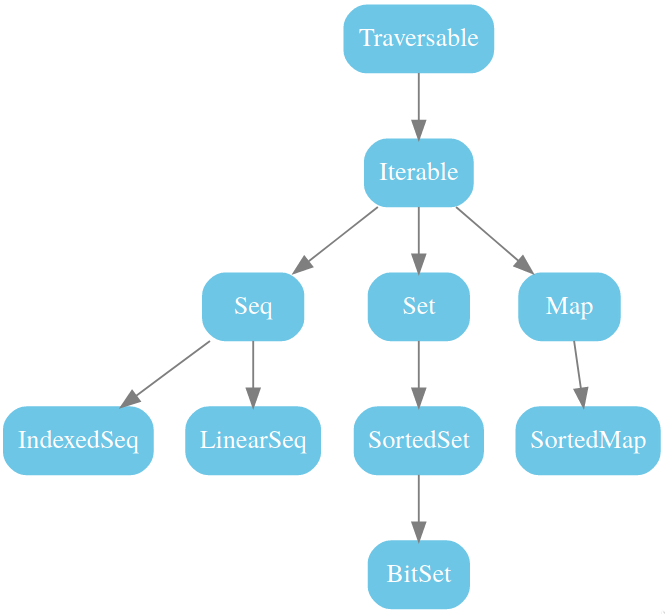
\includegraphics[scale=0.55]{../../img/collection/collection-traits}};

%
%
%\node[above right] (collection-traits) at ($(current page.west)+(1.0,7.5)$) {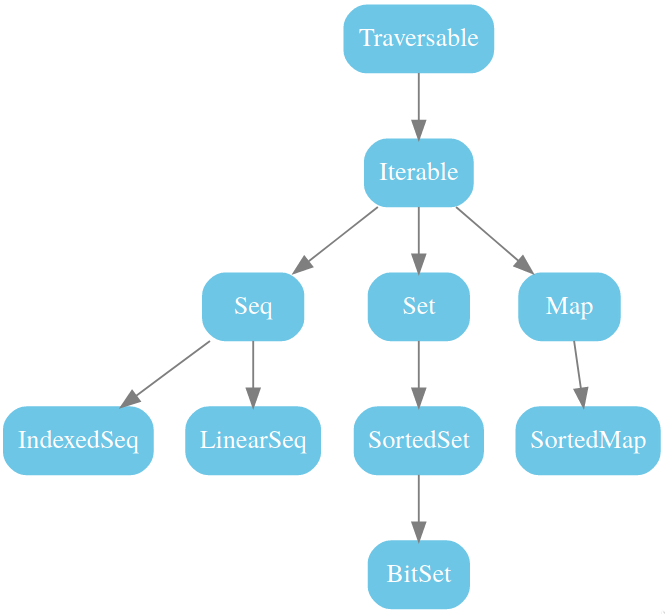
\includegraphics[scale=0.55]{../../img/collection/collection-traits}};
%
%\node[above right] (collection-traits-text) at ($(current page.west)+(1.0,12.5)$) {\texttt{\large scala.collection}};
%
%\node[above right] (collection-legend) at ($(current page.west)+(14.0,7.5)$) {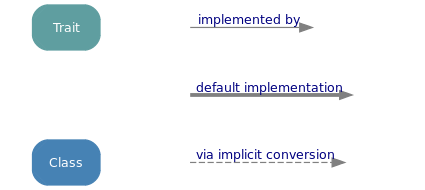
\includegraphics[scale=0.30]{../../img/collection/collection-legend}};
%
%\node[above right] (collection-immutable) at ($(current page.west)+(2,-3.4)$) {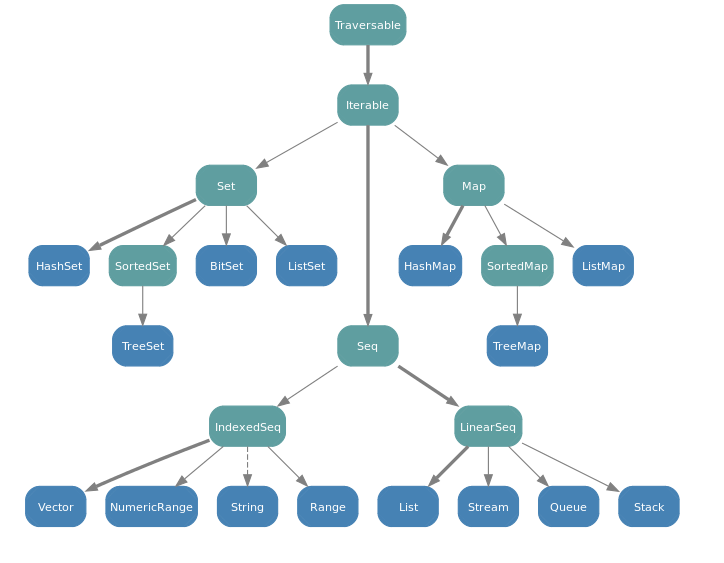
\includegraphics[scale=0.50]{../../img/collection/collection-immutable}};
%
%\node[above right] (collection-traits-text) at ($(current page.west)+(1.0,4.5)$) {\large\texttt{\large immutable}};
%
%\node[above right] (collection-mutable) at ($(current page.west)+(0,-15.2)$) {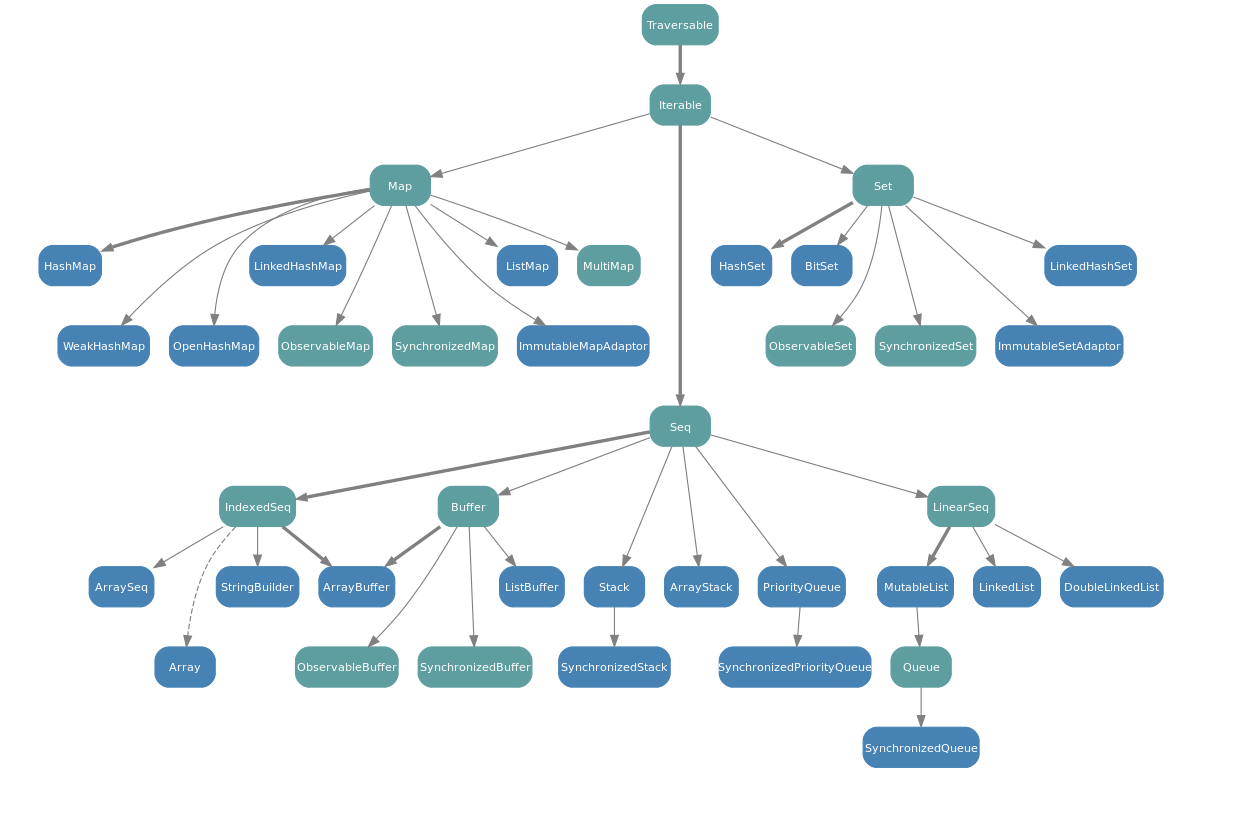
\includegraphics[scale=0.40]{../../img/collection/collection-mutable}};
%
%\node[above right] (collection-traits) at ($(current page.west)+(1.0,-5.5)$) {\texttt{\large mutable}};



% ../../img/collection/collection-immutable
\end{tikzpicture}
\end{document}
